%!TEX root = ../thesis.tex
% ******************************* Thesis Appendix B ********************************

\chapter{Smeared Truth Beam Bucket Distribution} 
\label{appendix_smeared}
\ifpdf
    \graphicspath{{Appendix6/Figs/Raster/}{Appendix6/Figs/PDF/}{Appendix6/Figs/}}
\else
    \graphicspath{{Appendix6/Figs/Vector/}{Appendix6/Figs/}}
\fi

\begin{figure}[b!]
        \begin{subfigure}[b]{0.495\textwidth}
            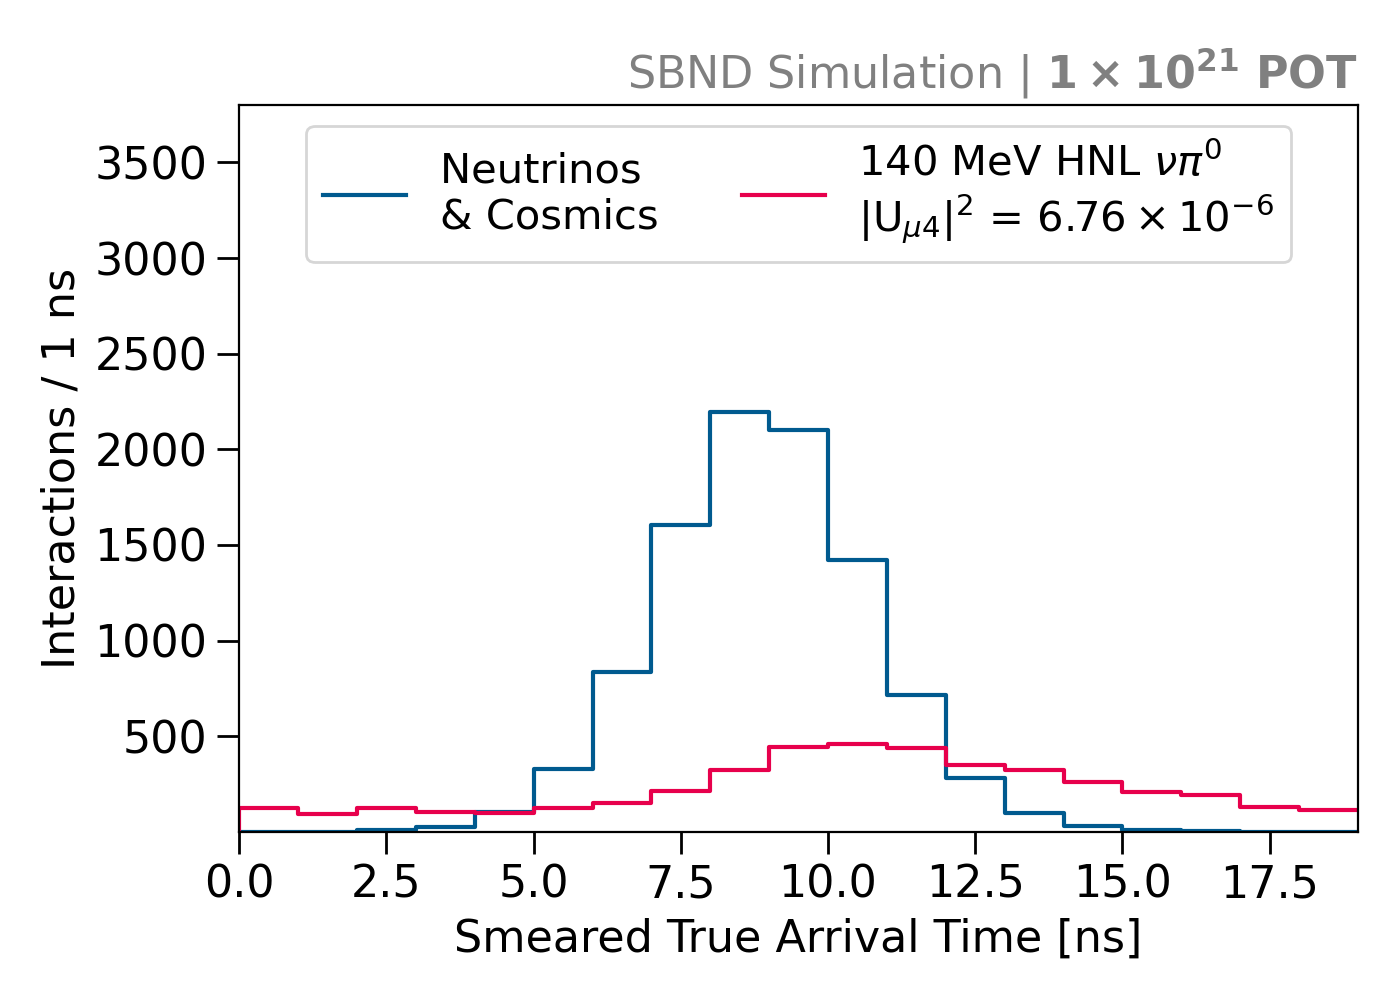
\includegraphics[width=\textwidth]{m140}
            \caption{$m_N = 140$ MeV, $|U_{\mu4}|^2 = 6.76 \times 10^{-6}$ }
        \end{subfigure}
        \begin{subfigure}[b]{0.495\textwidth}
            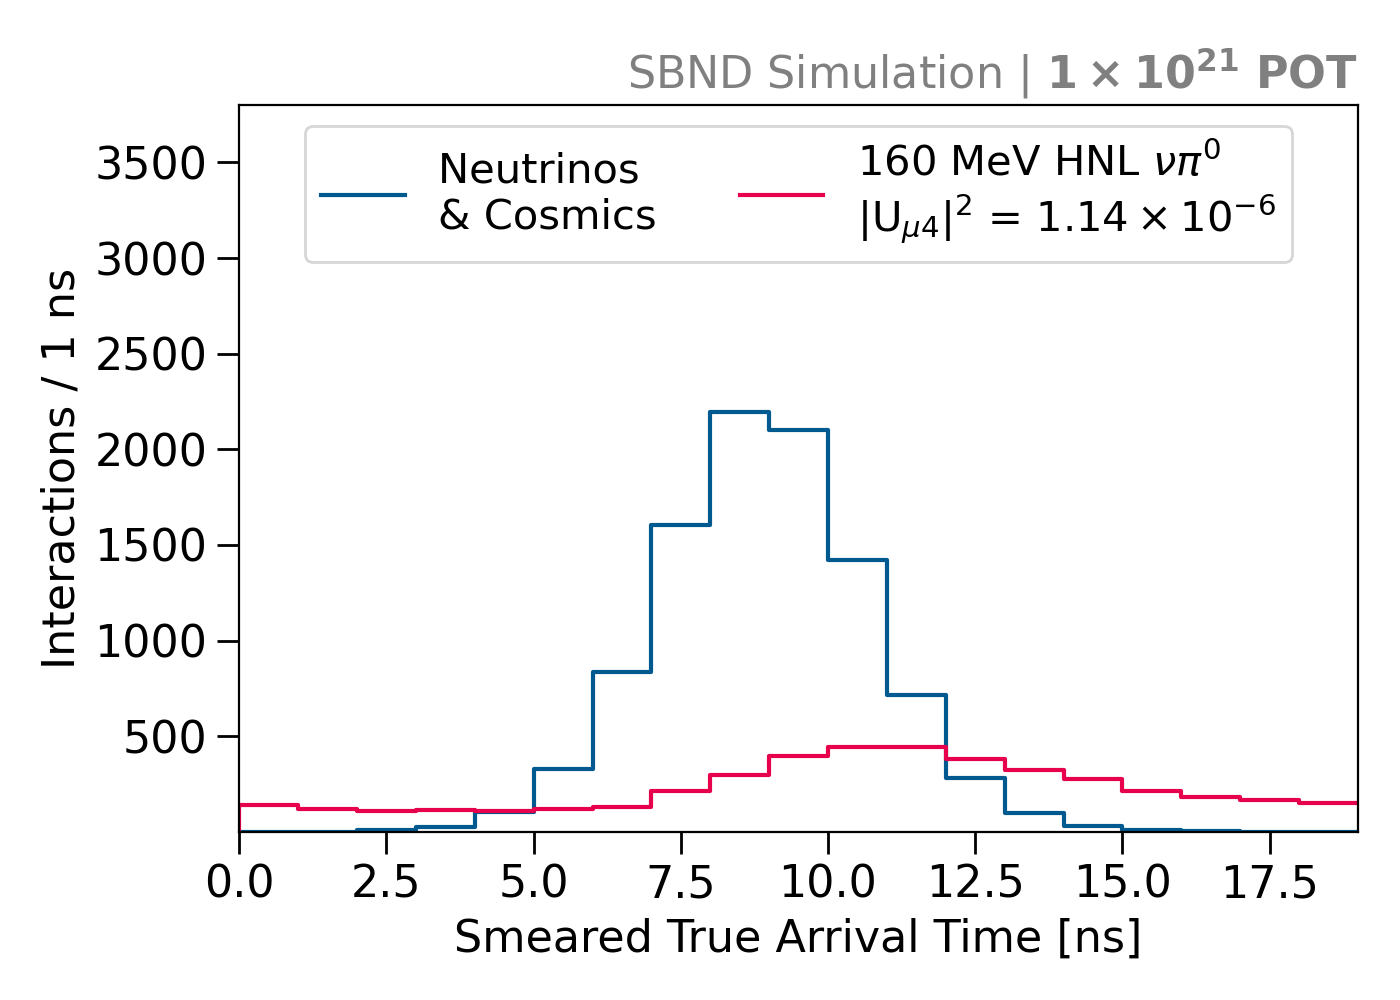
\includegraphics[width=\textwidth]{m160}
            \caption{$m_N = 160$ MeV, $|U_{\mu4}|^2 = 1.14 \times 10^{-6}$ }
        \end{subfigure}
        \begin{subfigure}[b]{0.495\textwidth}
            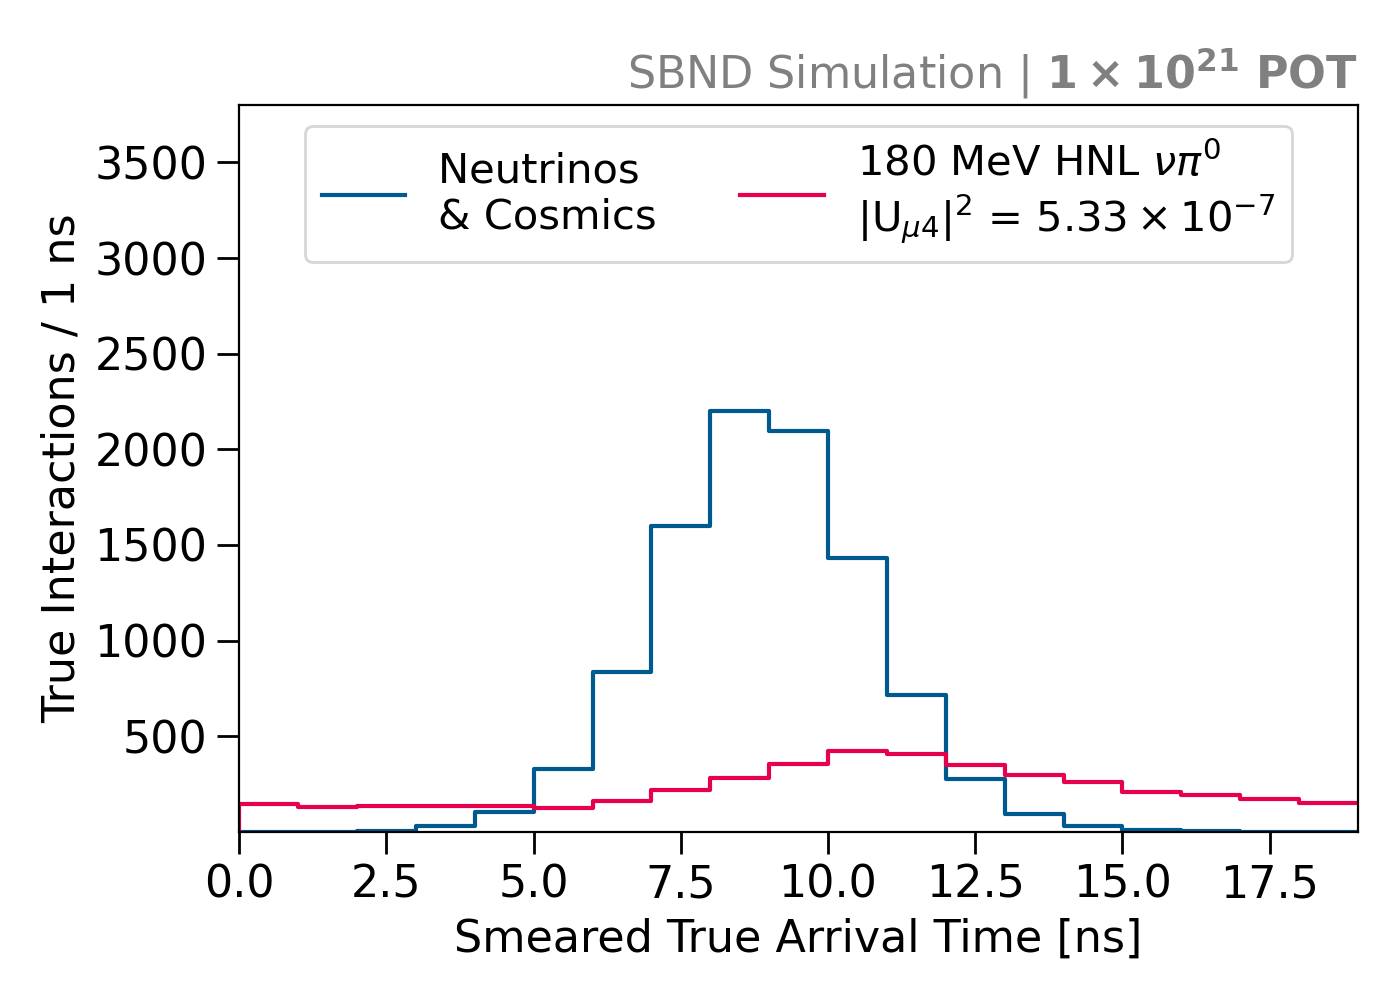
\includegraphics[width=\textwidth]{m180}
            \caption{$m_N = 180$ MeV, $|U_{\mu4}|^2 = 5.33 \times 10^{-7}$ }
        \end{subfigure}
        \begin{subfigure}[b]{0.495\textwidth}
            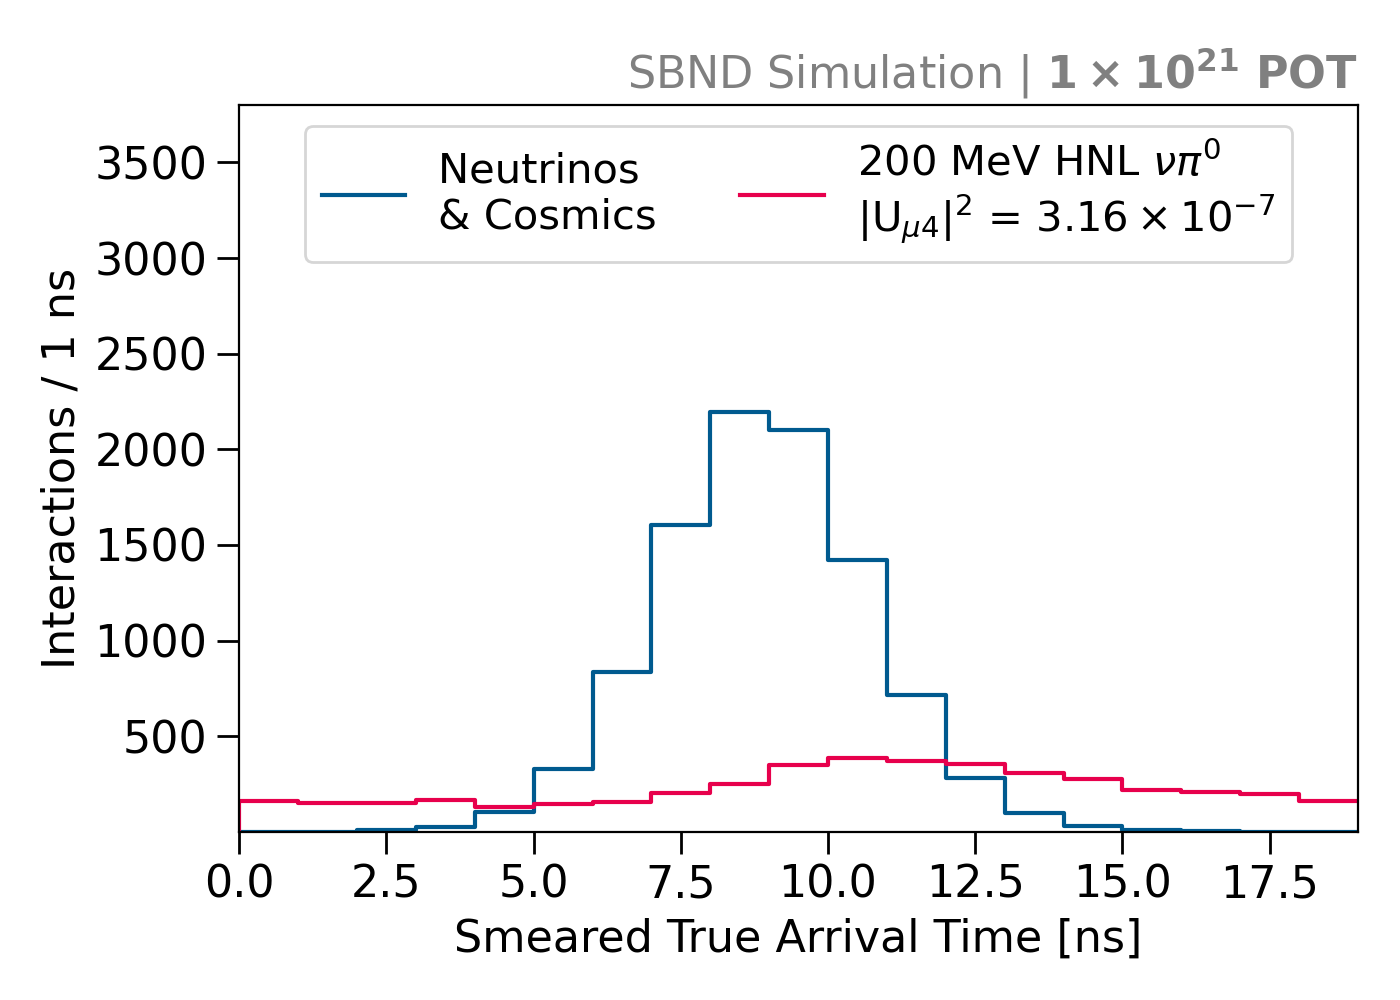
\includegraphics[width=\textwidth]{m200}
            \caption{$m_N = 200$ MeV, $|U_{\mu4}|^2 = 3.16 \times 10^{-7}$ }
        \end{subfigure}
        \caption[Smeared Truth Beam Bucket Distributions in the Mass Range 140 - 200 MeV]{
	Beam bucket distributions from smearing true arrival times.
	}
\end{figure}

\begin{figure}[hb!]
        \begin{subfigure}[b]{0.495\textwidth}
            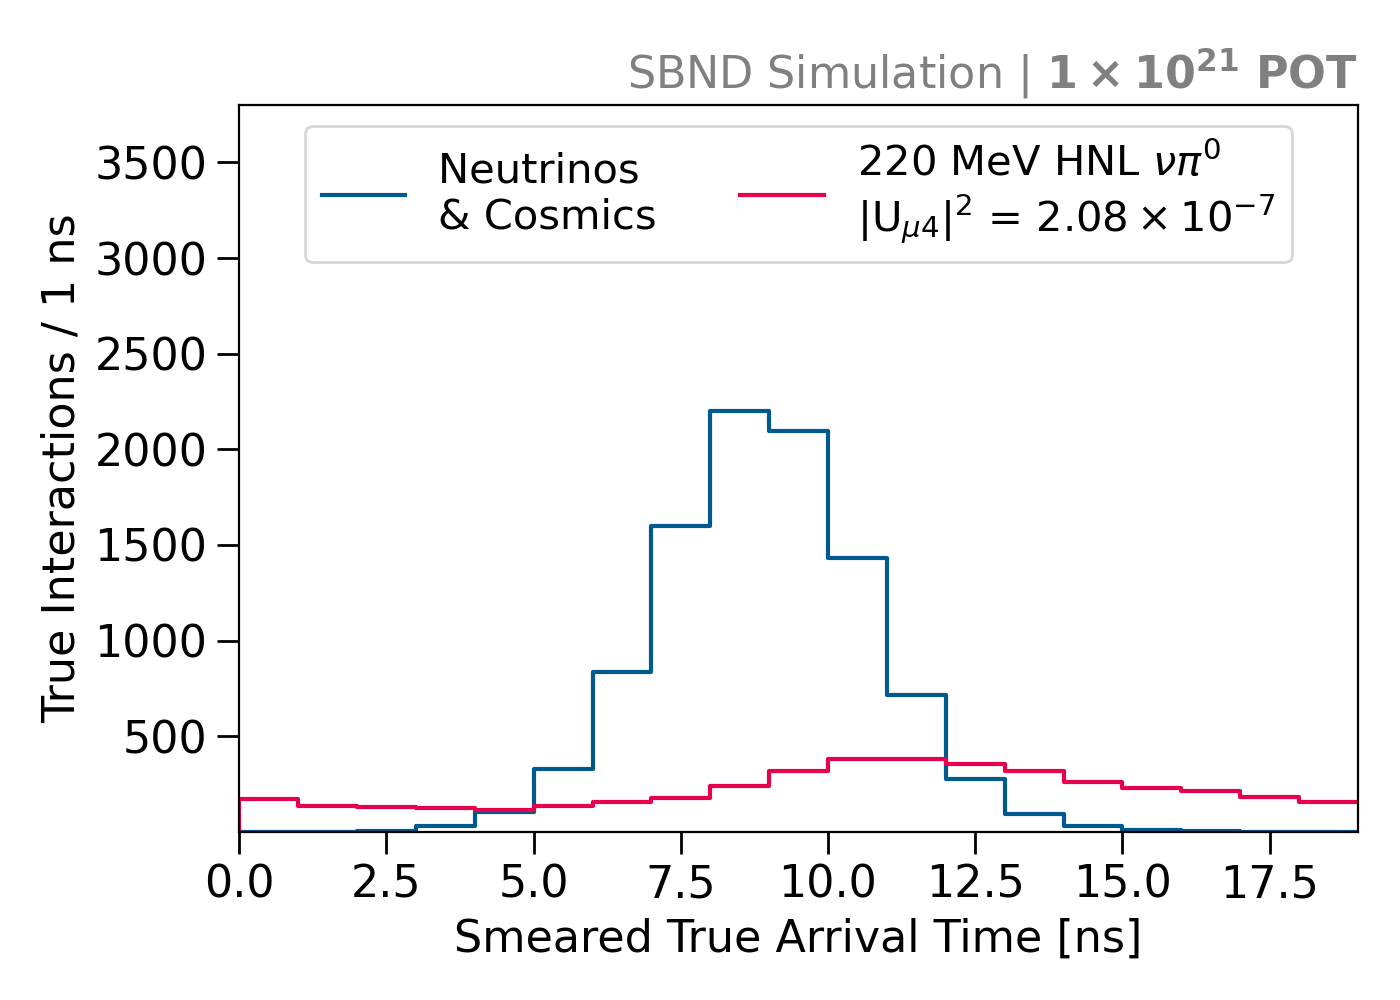
\includegraphics[width=\textwidth]{m220}
            \caption{$m_N = 220$ MeV, $|U_{\mu4}|^2 = 2.08 \times 10^{-7}$ }
        \end{subfigure}
	\hfill
        \begin{subfigure}[b]{0.495\textwidth}
            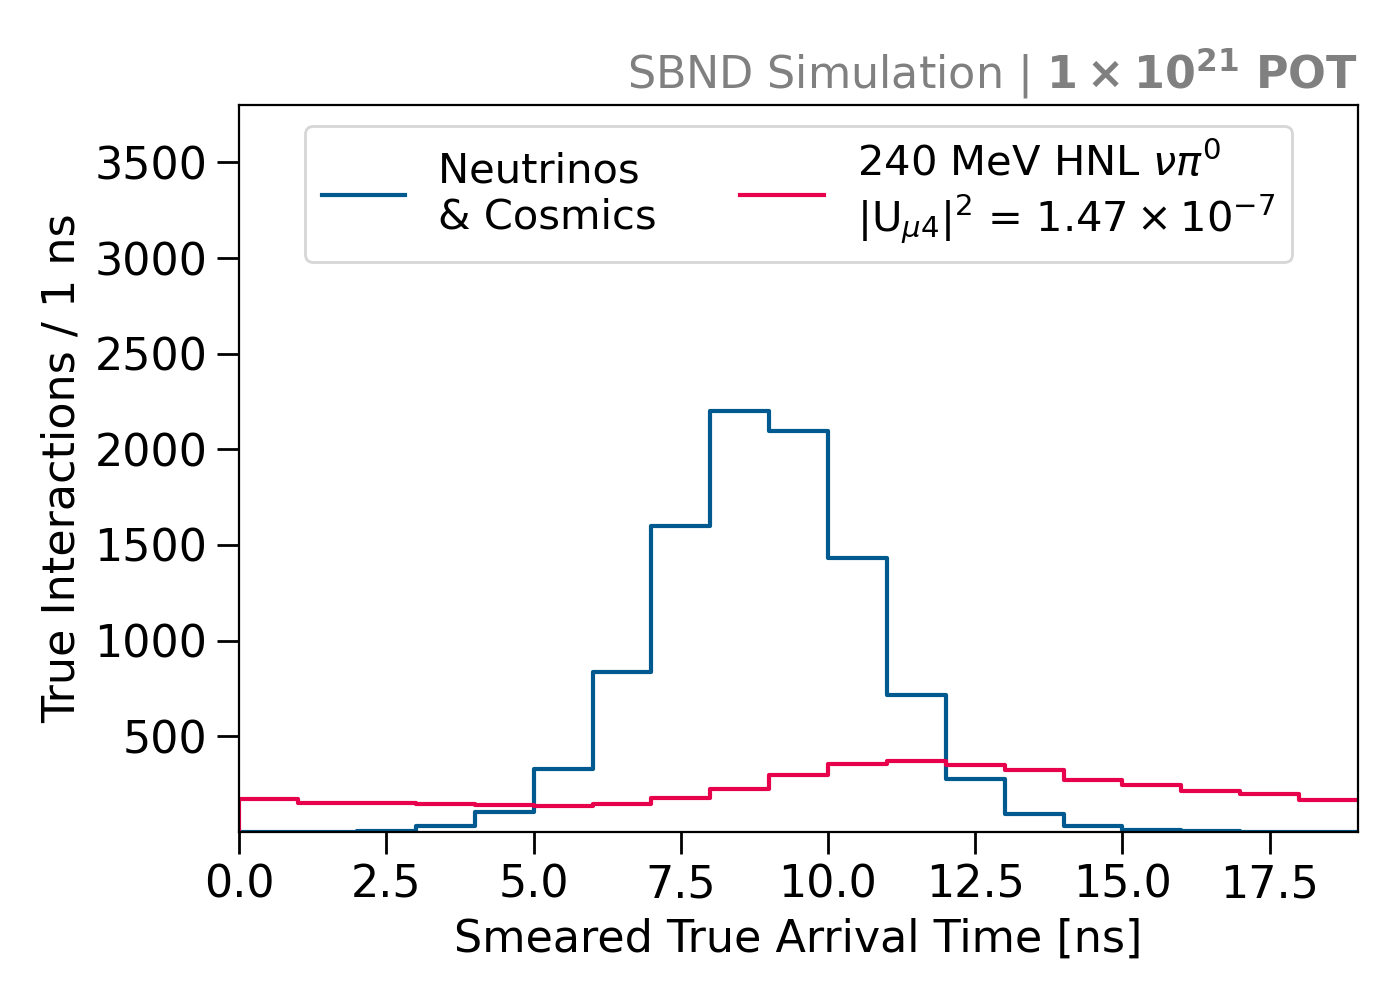
\includegraphics[width=\textwidth]{m240}
            \caption{$m_N = 240$ MeV, $|U_{\mu4}|^2 = 1.47 \times 10^{-7}$ }
        \end{subfigure}
	\centering
        \begin{subfigure}[b]{0.495\textwidth}
            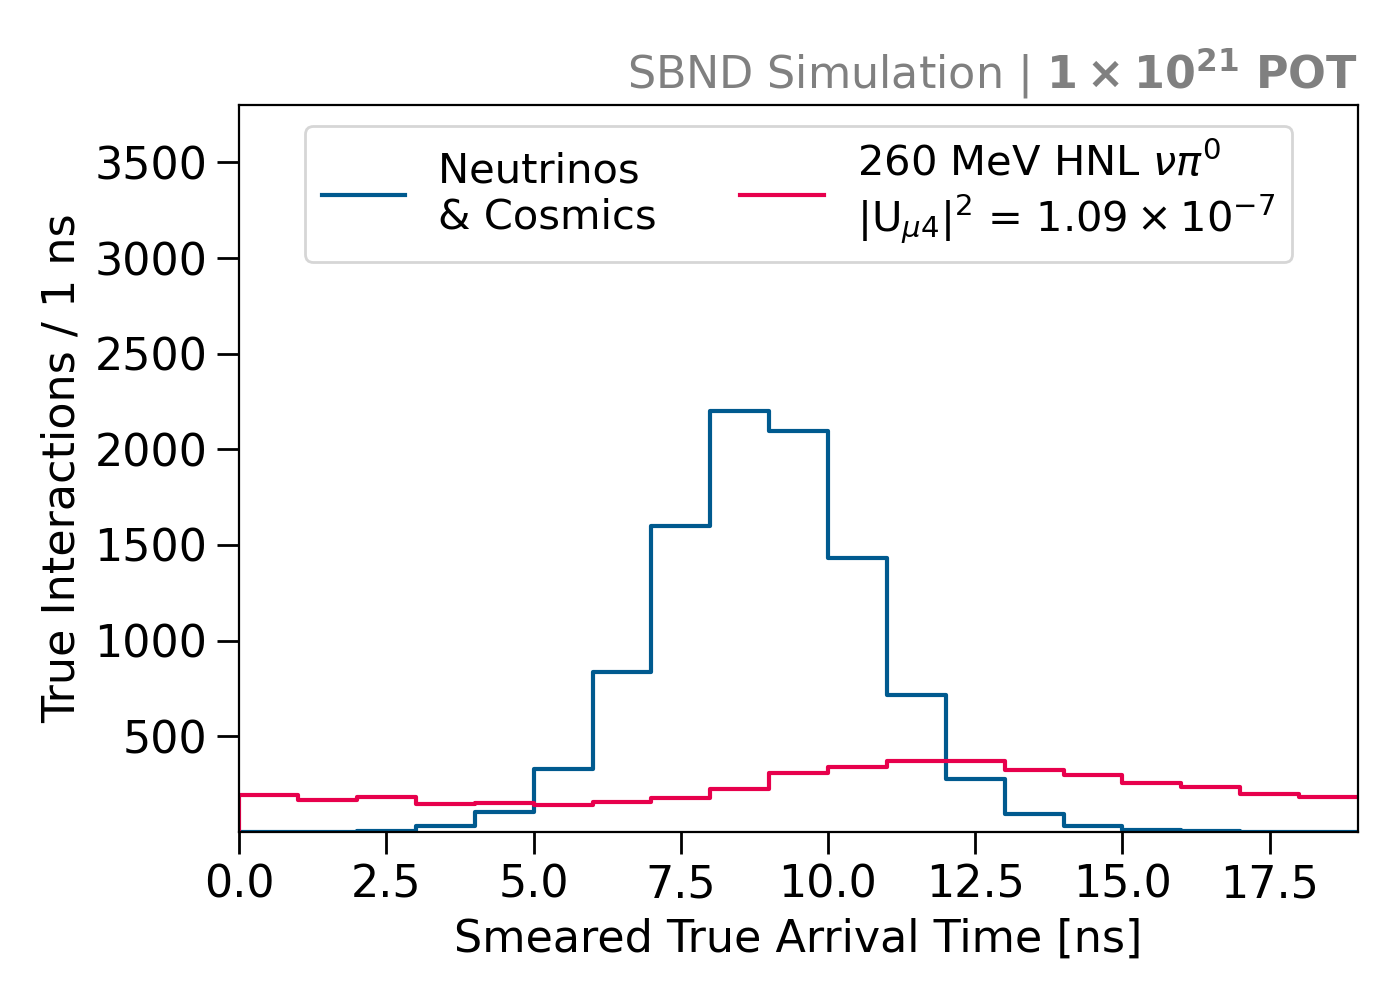
\includegraphics[width=\textwidth]{m260}
            \caption{$m_N = 260$ MeV, $|U_{\mu4}|^2 = 1.09 \times 10^{-7}$ }
        \end{subfigure}
        \caption[Smeared Truth Beam Bucket Distributions in the Mass Range 220 - 260 MeV]{
	Beam bucket distributions from smearing true arrival times.
	}
\end{figure}
